\documentclass[12pt]{article}
\usepackage[margin=1in]{geometry}
\usepackage{amsmath,amsthm,amssymb}

% Ignore spaces in filenames
\usepackage[space]{grffile}

\usepackage[T1]{fontenc}
\usepackage{bigfoot} % to allow verbatim in footnote
\usepackage[numbered,framed]{matlab-prettifier}
\usepackage{filecontents}
\usepackage{graphicx}
\usepackage[normalem]{ulem}

\let\ph\mlplaceholder % shorter macro
\lstMakeShortInline"

\lstset{
  style              = Matlab-editor,
  basicstyle         = \mlttfamily,
  escapechar         = ",
  mlshowsectionrules = true,
}

\title{MAE 275 - Homework 5}
\author{John Karasinski}

\begin{document}
\maketitle

\section{Defining the System}
The lateral linearized aircraft equations of motion can be expressed in state space form, with state variables $\Delta v, \Delta p, \Delta r, \Delta \varphi, \Delta \psi $, as
\begin{equation*}
A =
\begin{bmatrix}
    Y_v & Y_p & \left[ Y_r-u_0 \right] & g\cos \theta_0 & 0 \\
    L_v^\prime & L_p^\prime & L_r^\prime & 0 & 0 \\
    N_v^\prime & N_p^\prime & N_r^\prime & 0 & 0 \\
    0 & 1 & \tan \theta_0 & 0 & 0 \\
    0 & 0 & \sec \theta_0 & 0 & 0
\end{bmatrix}\\
\end{equation*}

\noindent Relevant B, C, and D matrices can also be formed
\begin{equation*}
B =
\begin{bmatrix}
     Y_{\delta_r}       & Y_{\delta_a} \\ 
     L_{\delta_r}^\prime & L_{\delta_a}^\prime \\
     N_{\delta_r}^\prime & N_{\delta_a}^\prime \\
     0           & 0 \\
     0           & 0 \\
\end{bmatrix}
\end{equation*}

\begin{equation*}
C =
\begin{bmatrix}
    1/u_0 & 0 & 0 & 0 & 0\\
    0     & 0 & 1 & 0 & 0\\
    0     & 0 & 0 & 1 & 0\\
\end{bmatrix}
\end{equation*}

\begin{equation*}
D =
\begin{bmatrix}
     0 & 0 \\
     0 & 0 \\
     0 & 0 \\
\end{bmatrix}
\end{equation*}

\noindent with $x = [\Delta v, \Delta p, \Delta r, \Delta \varphi, \Delta \psi]$ and $u =[\Delta \delta_r, \Delta \delta_a]$.

\noindent Plugging in the data for the DC-8 aircraft in Flight Condition 8002 from Appendix A of "Aircraft Dynamics and Automatic Control" yields
\begin{equation*}
A =
\begin{bmatrix}
  -1.0080e-1 &          0 & -4.6820e+2 & +3.2200e+1  &          0 \\
  -5.7881e-3 & -1.2320e+0 & +3.9700e-1 &          0  &          0 \\
  +2.7787e-3 & -3.4600e-2 & -2.5700e-1 &          0  &          0 \\
           0 &          1 &          0 &          0  &          0 \\
           0 &          0 &          1 &          0  &          0 \\

\end{bmatrix}
\end{equation*}

\begin{equation*}
B =
\begin{bmatrix}
  +1.3480e+1 &          0 \\
  +3.9200e-1 & -1.6200e+0 \\
  -8.6400e-1 & -1.8750e-2 \\
           0 &          0 \\
           0 &          0 \\
\end{bmatrix}
\end{equation*}

\begin{equation*}
C =
\begin{bmatrix}
   +2.1358e-3 &           0 &           0  &          0 &           0 \\
            0 &           0 &           1  &          0 &           0 \\
            0 &           0 &           0  &          1 &           0 \\
\end{bmatrix}
\end{equation*}

\begin{equation*}
D =
\begin{bmatrix}
     0  &   0 \\
     0  &   0 \\
     0  &   0 \\
\end{bmatrix}
\end{equation*}

% \clearpage
\section{Designing the Controllers}
Two controllers were designed. The first controller, $Gc_{\phi}$ was designed as
\begin{filecontents*}{code.m}
  -360.94 (s+1.413) (s+0.07616)
  -----------------------------
         s (s+100) (s+3)
\end{filecontents*}
\lstinputlisting[]{code.m}

\noindent This controller was determined using loop-shaping principles such that it had a roll-attitude bandwidth of $\sim$3 rad/sec (-3dB criterion) and a minimum overshoot in step response. \\

\begin{figure}[h!]
\begin{center}
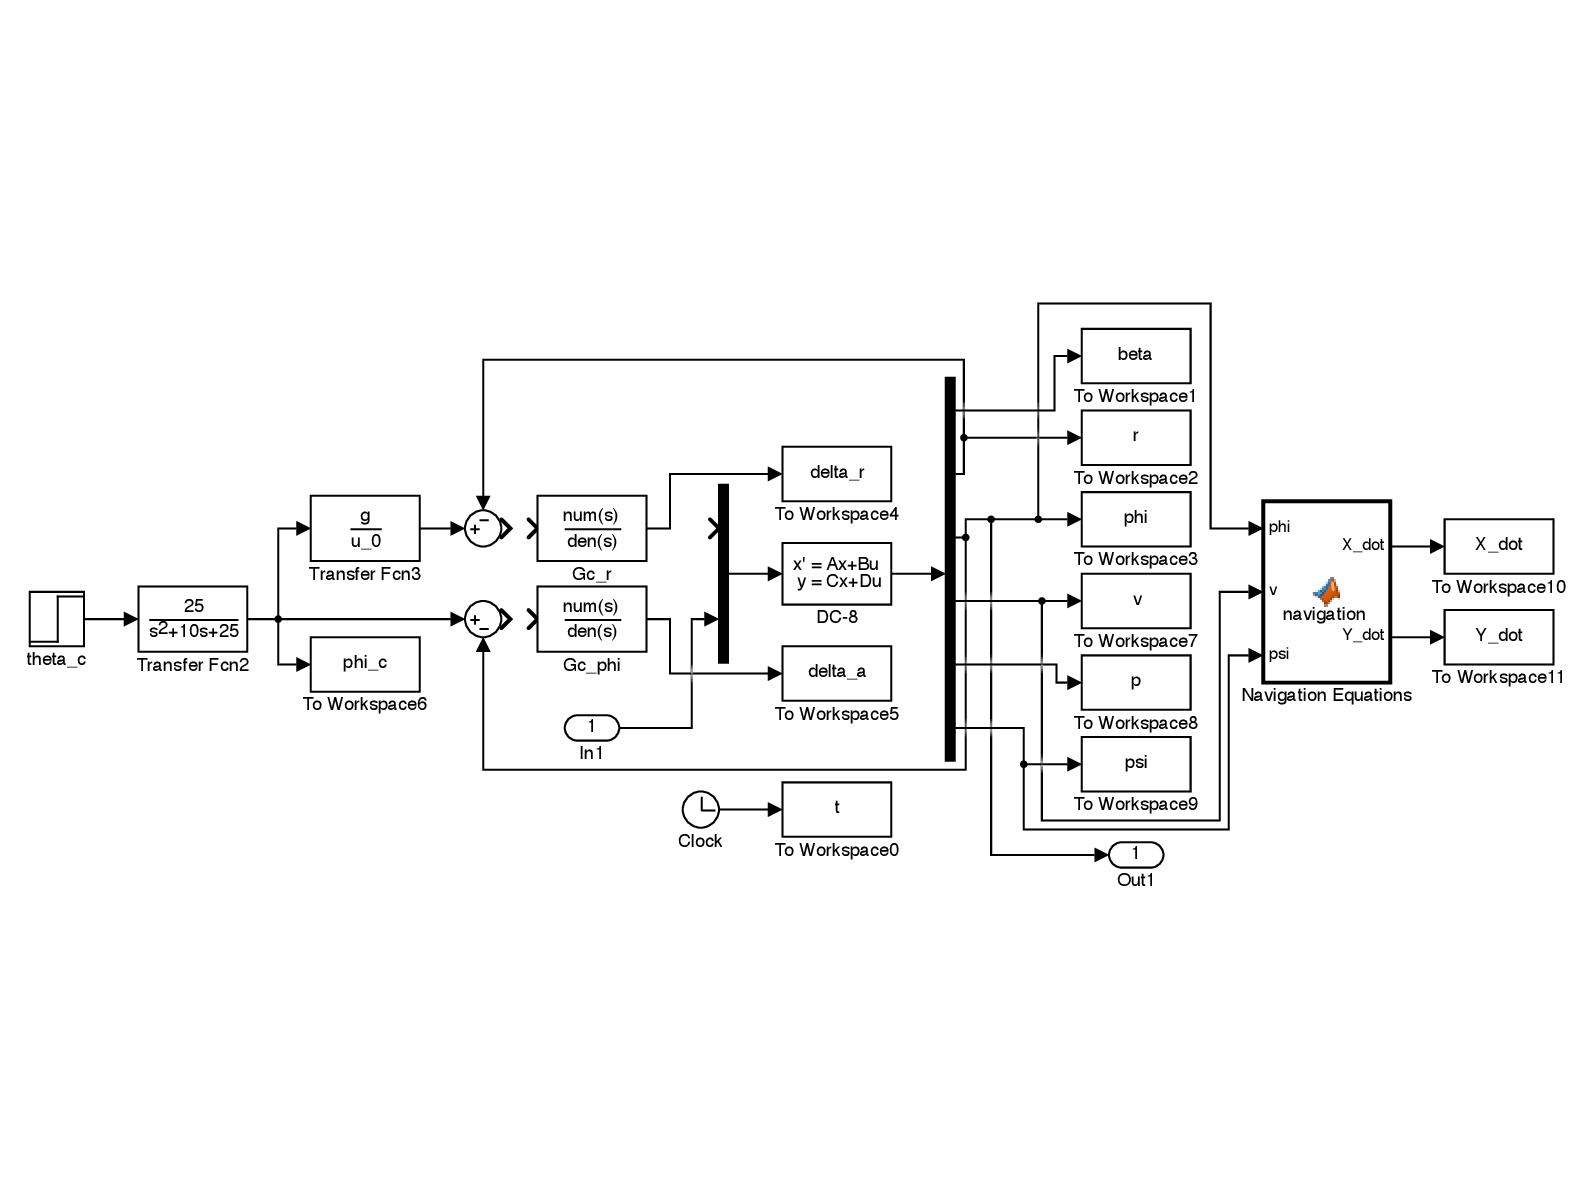
\includegraphics[height=.425\textheight]{figures/first_controller_simulink}
\caption{Simulink Diagram for First Controller Design}
\end{center}
\end{figure}

\noindent The second controller, $Gc_r$ was designed as
\begin{filecontents*}{code.m}
  21.969 (s-1.86)
  ----------------
  (s+10) (s+8.199)
\end{filecontents*}
\lstinputlisting[]{code.m}

\noindent This controller was determined using loop-shaping principles such that it had a bandwidth of $\sim$1 rad/sec (-3dB criterion), giving a factor of approximately three between r-loop and $\phi$-loop bandwidths. \\

\begin{figure}[h!]
\begin{center}
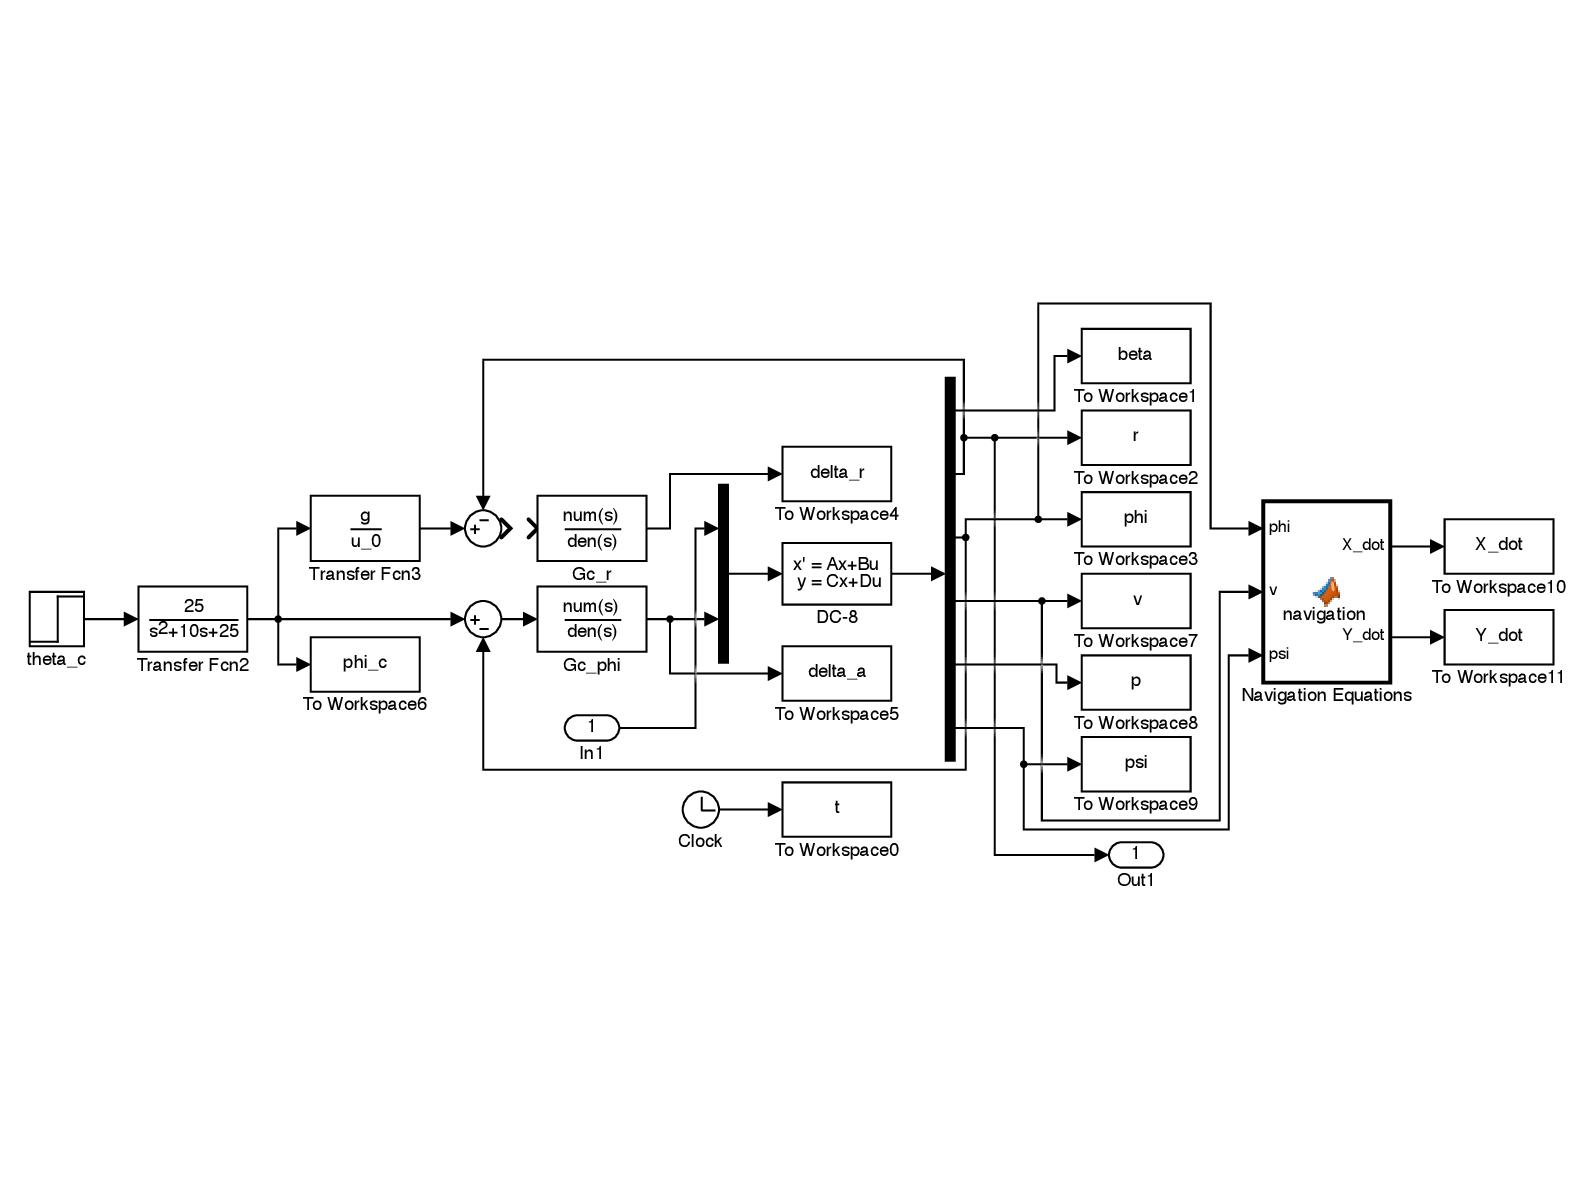
\includegraphics[height=.425\textheight]{figures/second_controller_simulink}
\caption{Simulink Diagram for Second Controller Design}
\end{center}
\end{figure}

\noindent Additionally, both controllers have:

more poles than zeros (are strictly proper compensators)

gain margins of at least 12dB

phase margins of at least 40 deg

\clearpage
\begin{figure}[h!]
\begin{center}
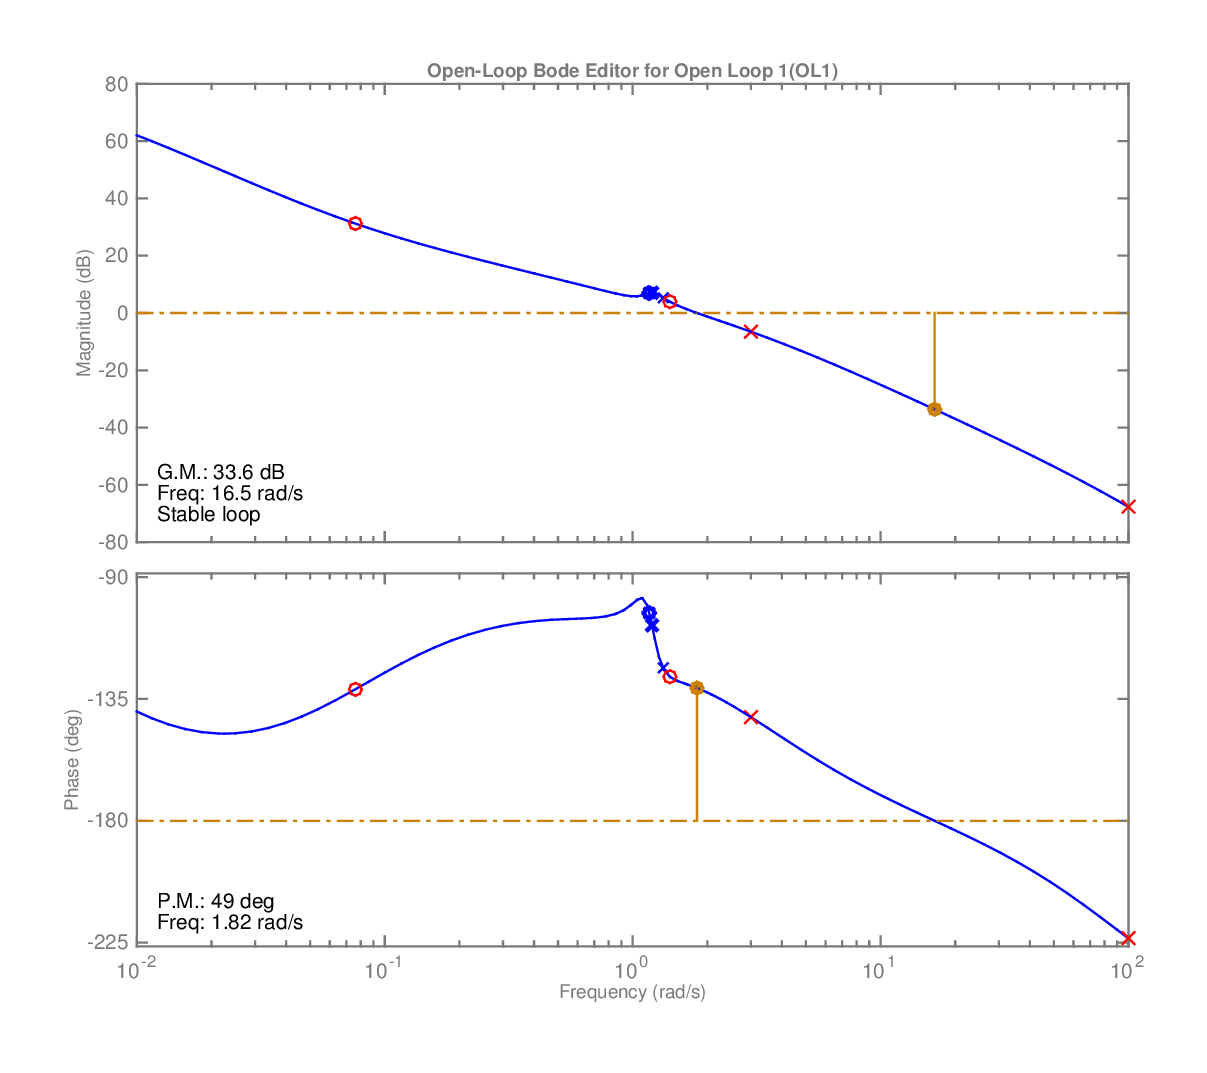
\includegraphics[height=.435\textheight]{figures/phi_delta_a_open_loop}
\caption{$\phi$-loop open-loop Bode with G.M. of 34 dB and P.M. of 49 deg}
\end{center}
\end{figure}

\begin{figure}[h!]
\begin{center}
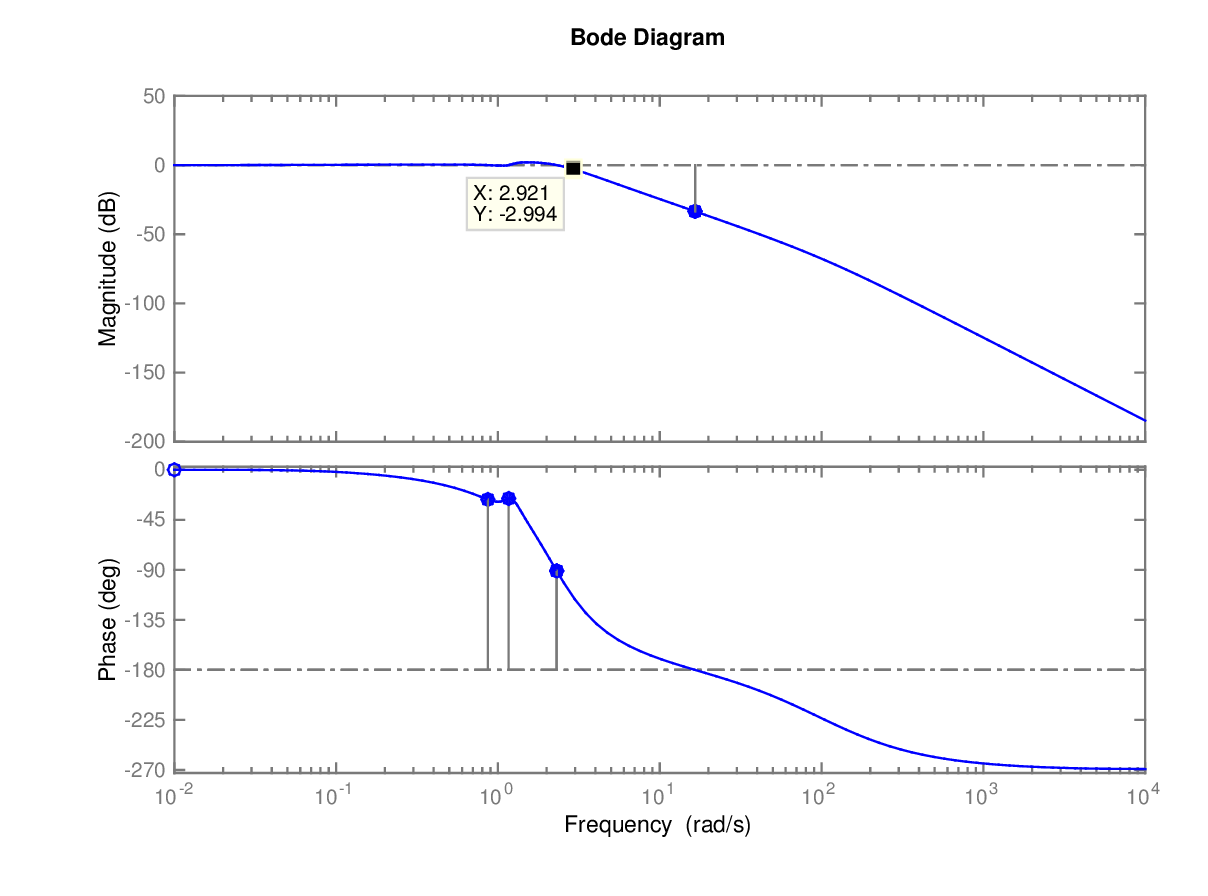
\includegraphics[height=.375\textheight]{figures/phi_delta_a_closed_loop}
\caption{$\phi$-loop closed-loop Bode with bandwidth of 3 rad/s (3dB criterion)}
\end{center}
\end{figure}

\begin{figure}[h!]
\begin{center}
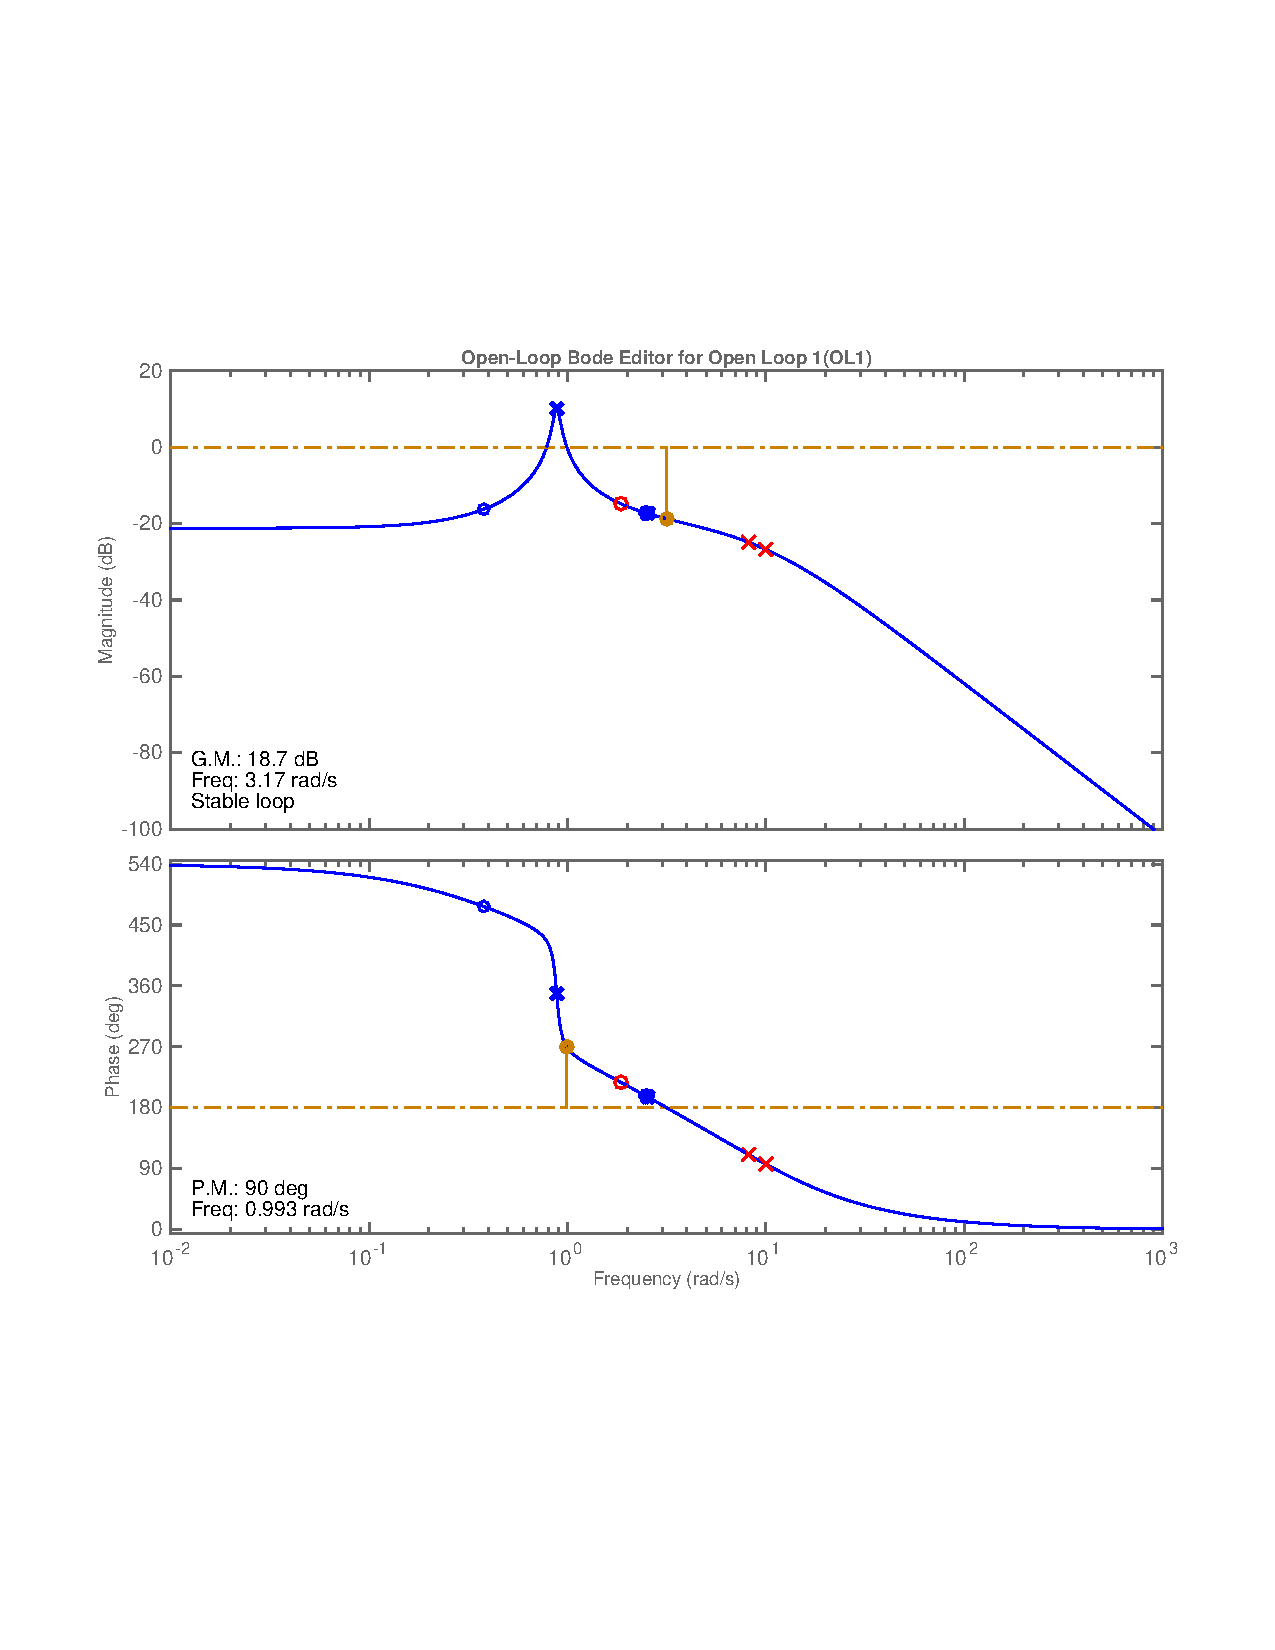
\includegraphics[height=.435\textheight]{figures/r_delta_r_open_loop}
\caption{$r$-loop open-loop Bode with G.M. of 18 dB and P.M. of 90 deg}
\end{center}
\end{figure}

\begin{figure}[h!]
\begin{center}
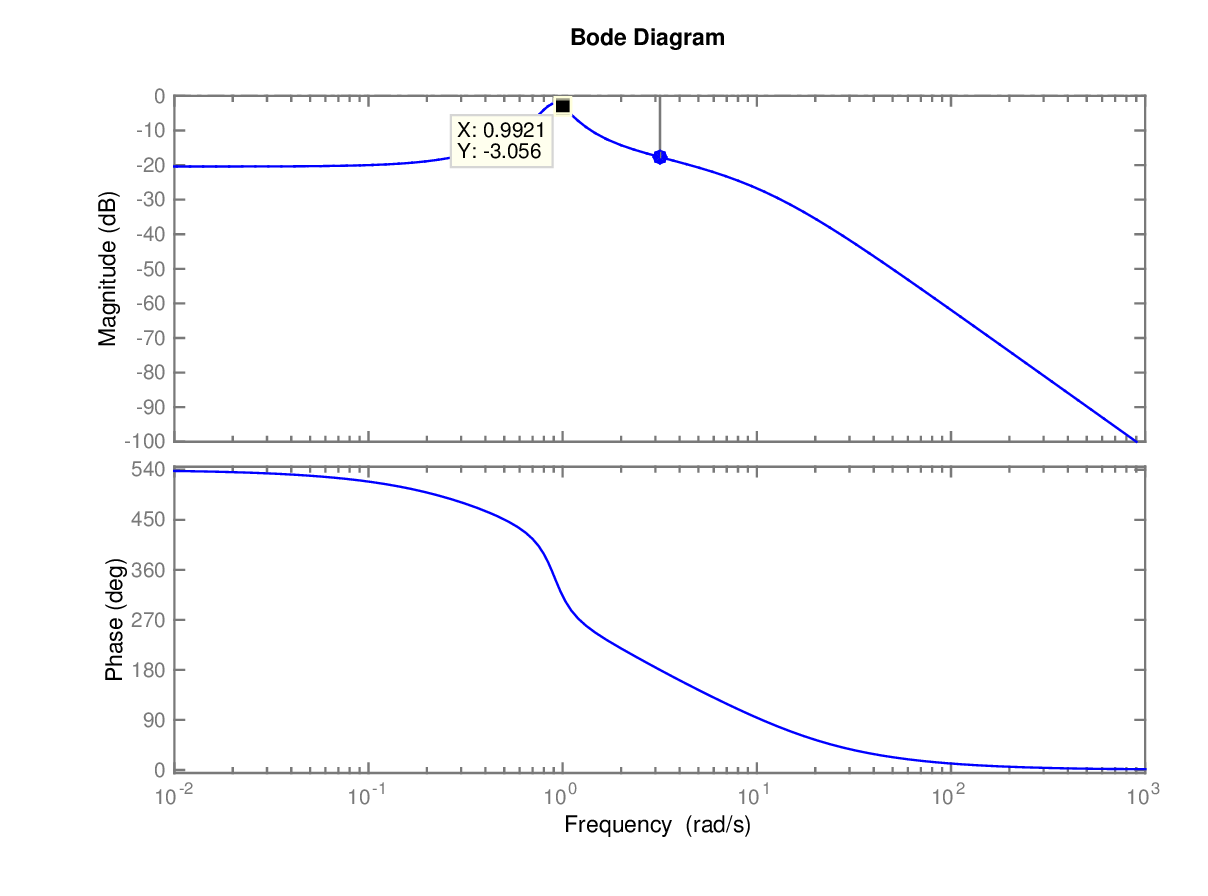
\includegraphics[height=.375\textheight]{figures/r_delta_r_closed_loop}
\caption{r-loop closed-loop Bode with bandwidth of 1 rad/s (3dB criterion)}
\end{center}
\end{figure}

\clearpage
\section{Final Simulink Diagram}
\begin{figure}[h!]
\begin{center}
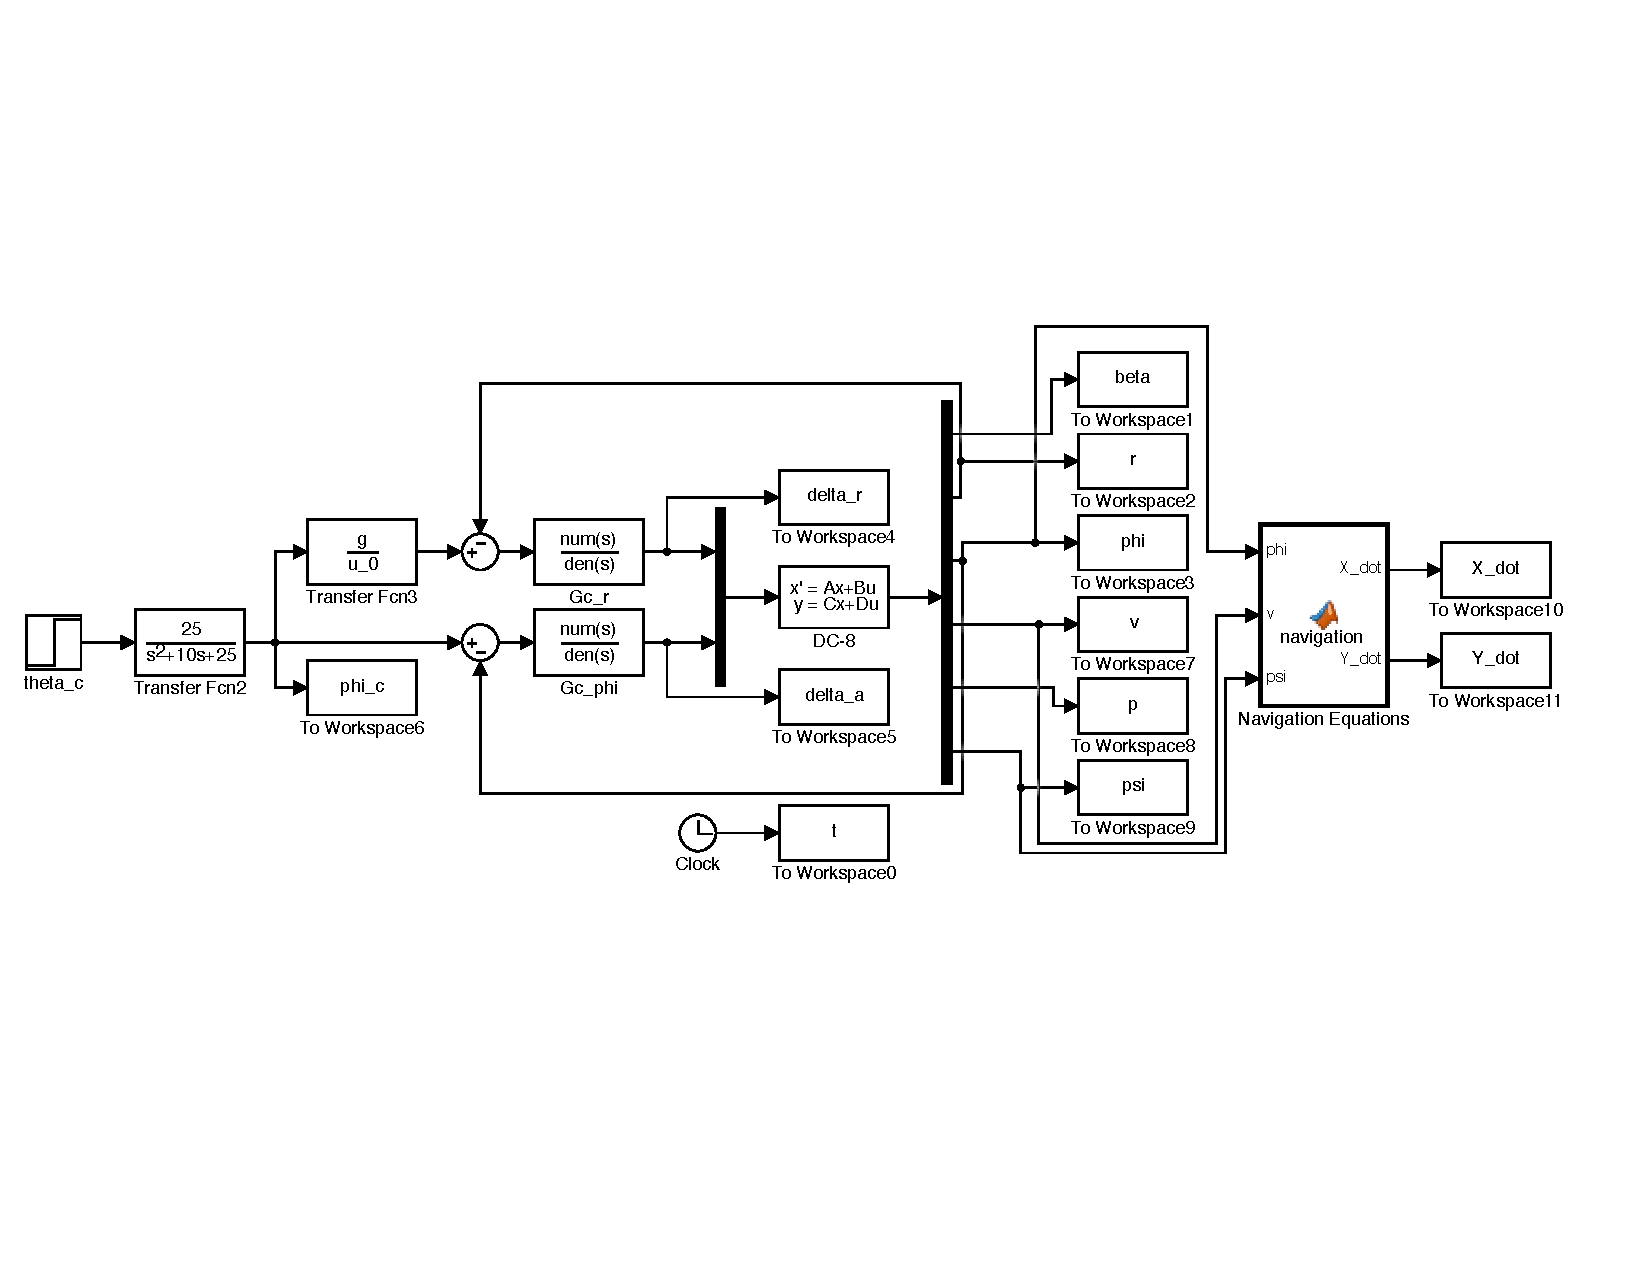
\includegraphics[width=1\textwidth]{figures/final_simulink}
\caption{Simulink Diagram}
\end{center}
\end{figure}

\noindent Where the navigation function is defined as
\begin{filecontents*}{code.m}
function [X_dot, Y_dot] = navigation(phi, v, psi)
%#codegen

theta = 0;
U = 468.2;
V = v;
W = 0;

X_dot = U * (cos(psi) * cos(theta)) + ...
        V * (cos(psi) * sin(theta) * sin(phi) - sin(psi) * cos(phi)) + ...
        W * (cos(psi) * sin(theta) * cos(phi) + sin(psi) * sin(phi));

Y_dot = U * (sin(psi) * cos(theta)) + ...
        V * (sin(psi) * sin(theta) * sin(phi) - cos(psi) * cos(phi)) + ...
        W * (sin(psi) * sin(theta) * cos(phi) + cos(psi) * sin(phi));
\end{filecontents*}
\lstinputlisting[]{code.m}

\clearpage
\section{Results}

\begin{figure}[h!]
\begin{center}
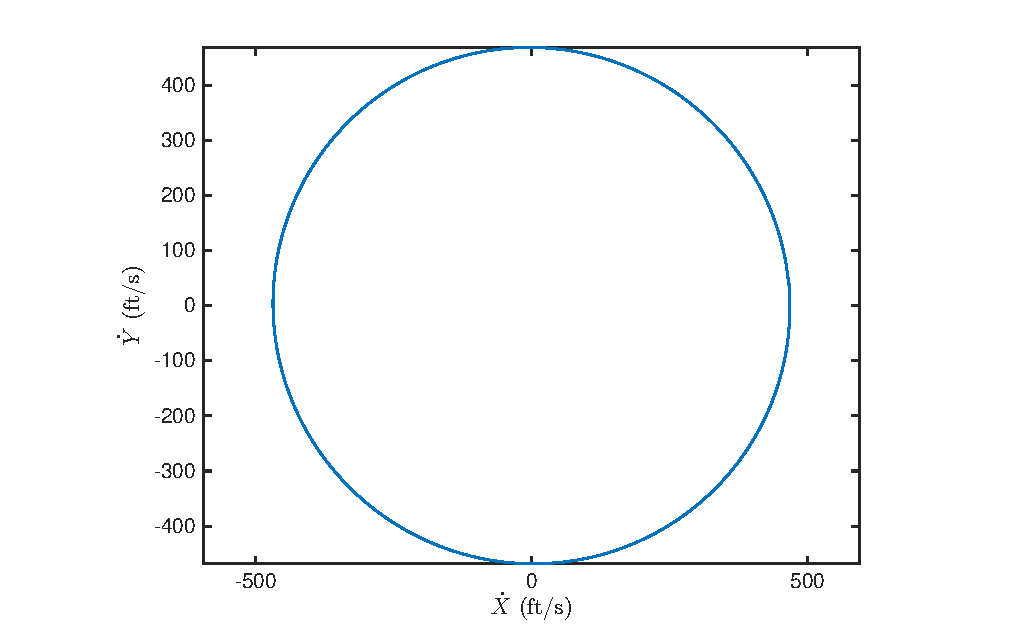
\includegraphics[width=.85\textwidth]{figures/circle}
\caption{Demonstration of turn-coordination from $\sim$ 267 second simulation}
\end{center}
\end{figure}

\begin{figure}[h!]
\begin{center}
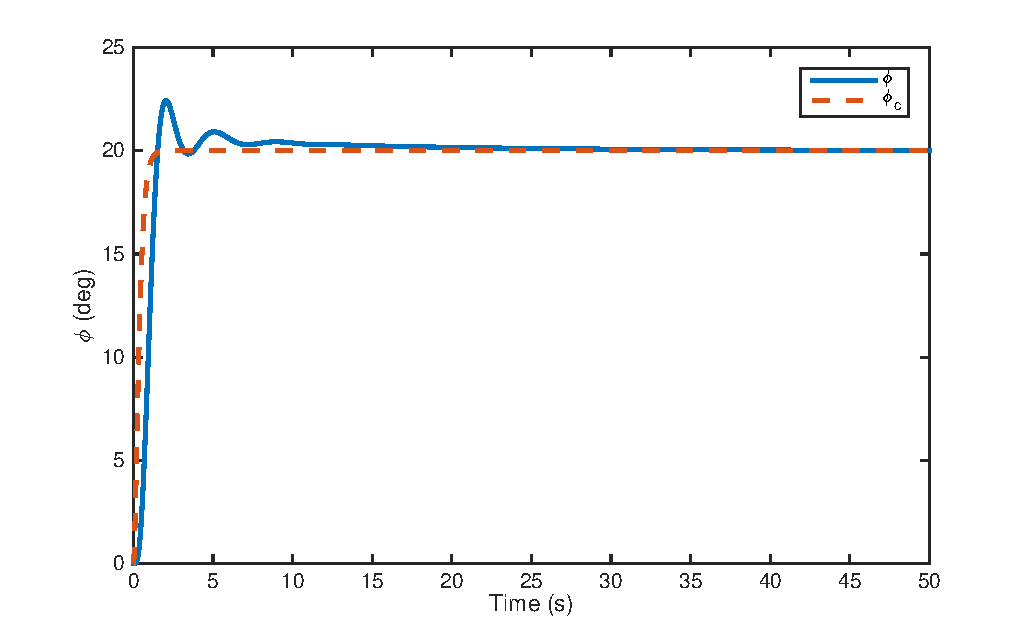
\includegraphics[width=.85\textwidth]{figures/phi}
\caption{$\phi$ response to $\phi_c$, showing $\sim 10\%$ overshoot}
\end{center}
\end{figure}

\clearpage
\begin{figure}[h!]
\begin{center}
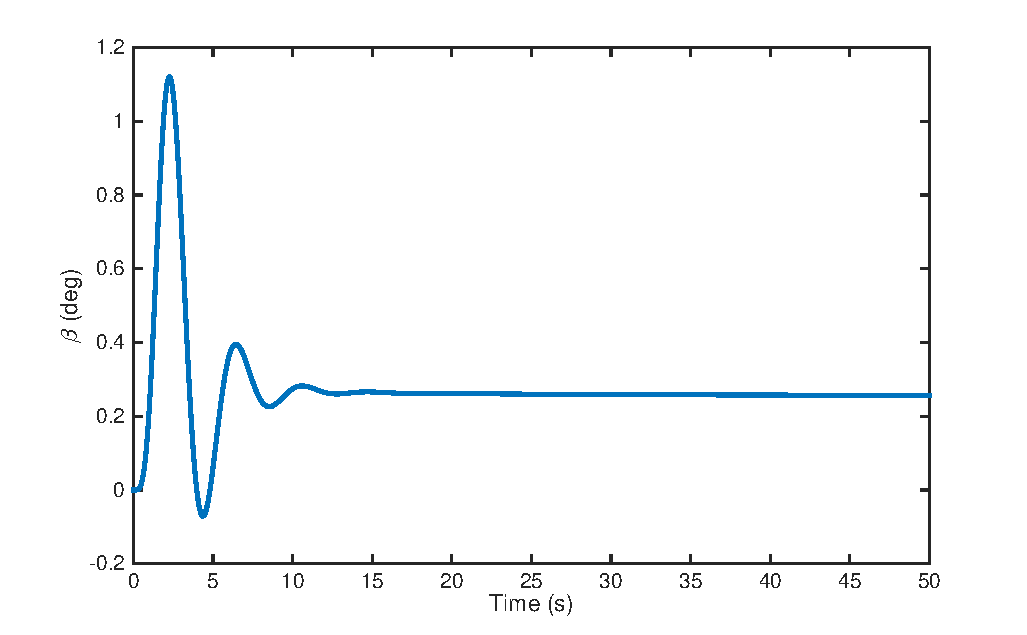
\includegraphics[height=.4\textheight]{figures/beta}
\caption{$\beta$ Response}
\end{center}
\end{figure}

\begin{figure}[h!]
\begin{center}
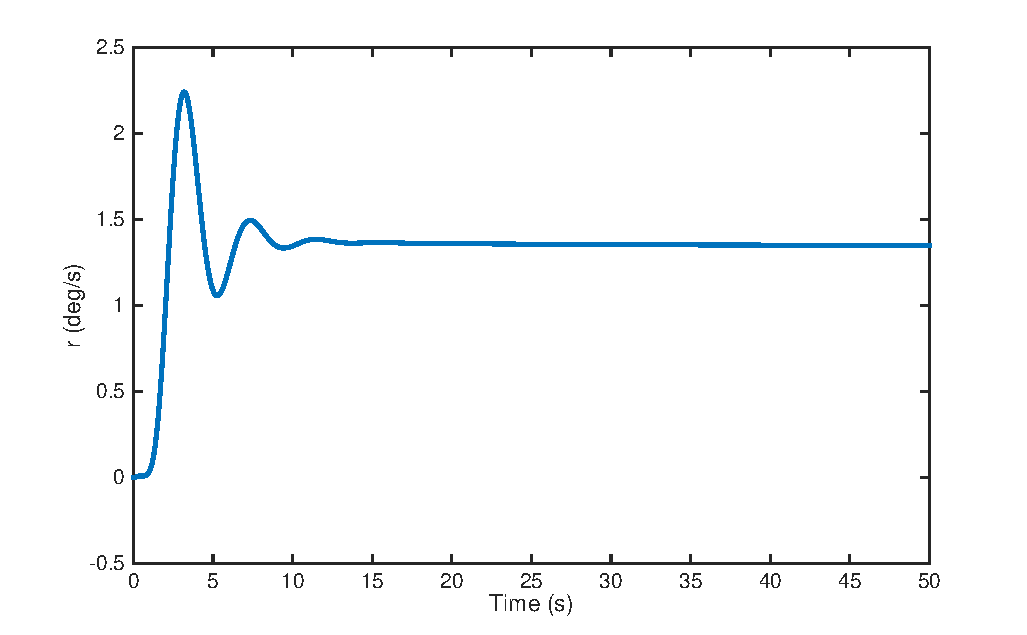
\includegraphics[height=.4\textheight]{figures/r}
\caption{$r$ Response}
\end{center}
\end{figure}

\clearpage
\begin{figure}[h!]
\begin{center}
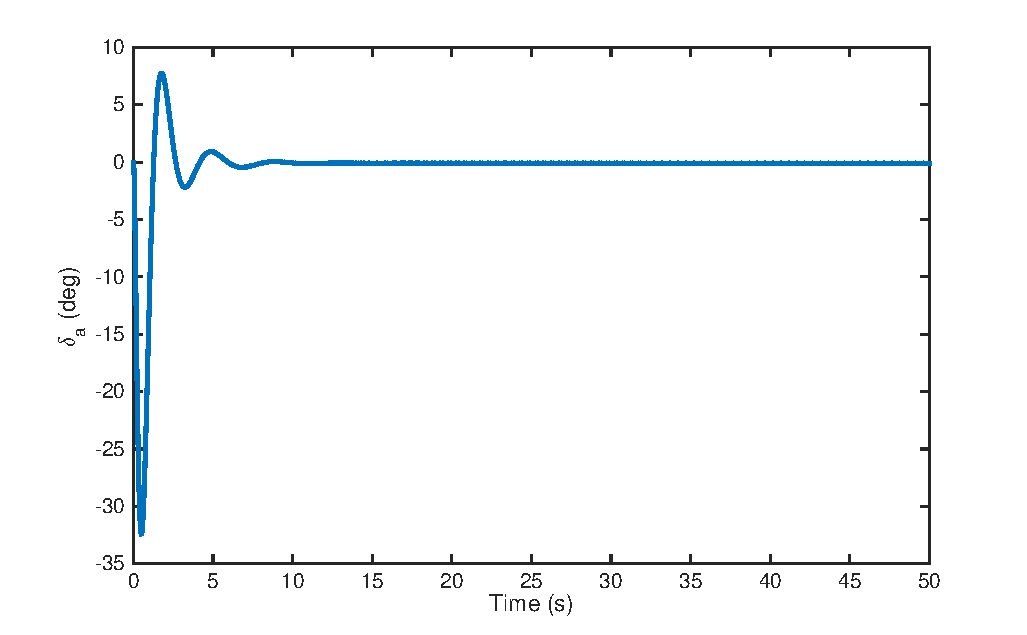
\includegraphics[height=.4\textheight]{figures/delta_a}
\caption{$\delta_a$ Input}
\end{center}
\end{figure}

\begin{figure}[h!]
\begin{center}
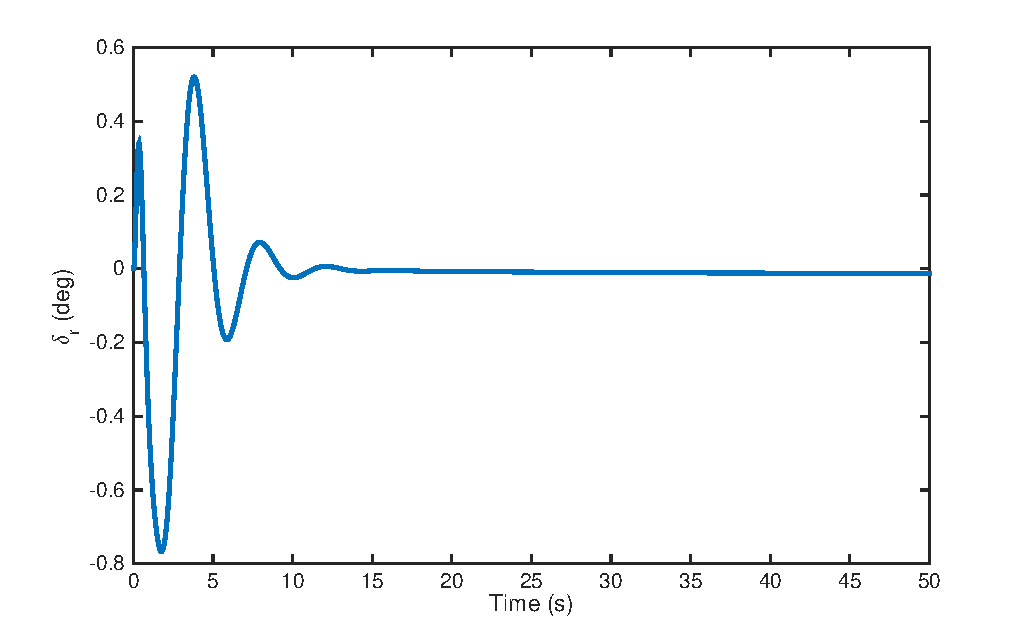
\includegraphics[height=.4\textheight]{figures/delta_r}
\caption{$\delta_r$ Input}
\end{center}
\end{figure}

\end{document}
